\documentclass[]{article}
\usepackage[utf8]{inputenc}
\usepackage[english,russian]{babel}
%\usepackage[12pt]{extsizes}
\usepackage{amsmath}
\usepackage{enumerate}

%\usepackage[left=3cm, top=1.5cm, right=1.3cm, bottom=2cm, nohead, footskip=10mm]{geometry}
\usepackage[12pt]{extsizes}
\linespread{1.3}
\usepackage[left=3cm, top=1.5cm, right=1.3cm, bottom=2cm, nohead, footskip=10mm]{geometry}


\usepackage[absolute,overlay]{textpos}
\usepackage{indentfirst}
\usepackage{float}
\restylefloat{table}
\usepackage{hyperref}
\usepackage{mathtext}
\usepackage{amsfonts}
\usepackage{amsthm}
\usepackage{tikz}
\usepackage{xspace}
\usetikzlibrary{shapes,positioning,shadows,trees,automata,arrows.meta,shapes.geometric}
\usepackage{pgf-pie}
\usepackage{chngcntr}
\usepackage{pdfpages}
\usepackage{systeme}
\usepackage{empheq}
\numberwithin{equation}{section}
\usepackage{caption}
\DeclareCaptionLabelSeparator{none}{. }
\captionsetup{labelsep=none}


\pagestyle{plain}

\renewcommand{\labelenumii}{\theenumii}
\renewcommand{\theenumii}{\arabic{enumii}.}

\begin{document}
    \thispagestyle{empty}
	\begin{center}
		Министерство образования и науки Российской Федерации\\
		Санкт-Петербургский государственный технический университет\\
		Институт прикладной математики и механики\\
		Кафедра <<Телематика>>\\
		\vspace{5cm}
		\textbf{\textbf{ЛАБОРАТОРНАЯ РАБОТА}}\\
        \vspace{0.5cm}
        \textbf{ПО ТЕМЕ}\\
        \vspace{0.5cm}
		\textbf{\textbf{<<Метод опорных векторов>>}}\\
		\vspace{3cm}
		по направлению 02.04.01.02 <<Организация и управление суперкомпьютерными системами>>
	\end{center}
	\vspace{2cm}
	\begin{tabular} {l l l}
	\hspace{9.5cm} & Выполнил: & \\
	& Студент гр. 13643.1 & Титов А.И.\\
	& Проверил: & Уткин Л.В.
	\end{tabular}
	\vspace{4.5cm}
	\begin{center}
		Санкт-Петербург\\
		2019
    \end{center}


	\renewcommand\contentsname{Оглавление}
	\tableofcontents

    \newpage
    \section*{Постановка задачи}
    \addcontentsline{toc}{section}{Постановка задачи}

    Требуется выполнить следующие задачи:
    \begin{enumerate}
        \item Постройте алгоритм метода опорных векторов типа <<C-classification>> с параметром C = 1, используя ядро <<linear>>. Визуализируйте разбиение пространства признаков на области с помощью полученной модели. Выведите количество полученных опорных векторов, а также ошибки классификации на обучающей и тестовой выборках.
        \item Используя алгоритм метода опорных векторов типа <<C-classification>> с линейным ядром, добейтесь нулевой ошибки сначала на обучающей выборке, а затем на тестовой, путем изменения параметра C.
        \item Среди ядер <<polynomial>>, <<radial>> и <<sigmoid>> выберите оптимальное в плане количества ошибок на тестовой выборке. Попробуйте различные значения параметра degree для полиномиального ядра.
        \item Среди ядер <<polynomial>>, <<radial>> и <<sigmoid>> выберите оптимальное в плане количества ошибок на тестовой выборке.
        \item Среди ядер <<polynomial>>, <<radial>> и <<sigmoid>> выберите оптимальное в плане количества ошибок на тестовой выборке. Изменяя значение параметра gamma, продемонстрируйте эффект переобучения, выполните при этом визуализацию разбиения пространства признаков на области.
        \item Постройте алгоритм метода опорных векторов типа <<eps-regression>> с параметром C = 1, используя ядро <<radial>>. Отобразите на графике полученные точки обучающей выборки, опорные векторы, восстановленную зависимость и ее $\epsilon$-окрестность.
    \end{enumerate}

    Данные для обучения и тестирования SVM-моделей, которые необходимо построить в приведенных выше заданиях, хранятся в файлах с именами svmdataI.txt и svmdataItest.txt, где I номер задания.

    \newpage
    \section{Набор данных <<svmdata1>>}
        На основе метода опорных векторов типа <<C-classification>> был построен классификатор с параметром C = 1 и ядром <<linear>>. Были построены графики разбиения пространства для обучающей и тестирующих выборок (рис. 1).
        \vspace{-0.5cm}
        \begin{figure}[H]
            \centering
            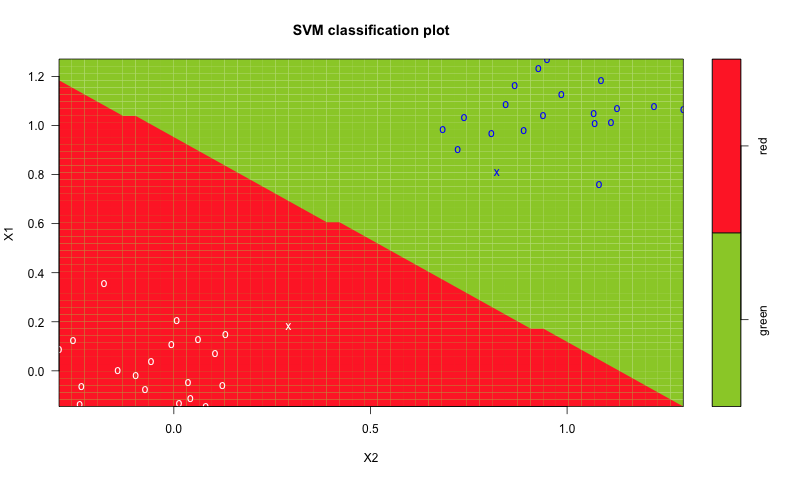
\includegraphics[width = 0.9\linewidth]{data/data1_train_set.png}
            \caption{Разбиение пространства для обучающей выборки}
        \end{figure}
        \vspace{-1cm}
        \begin{figure}[H]
            \centering
            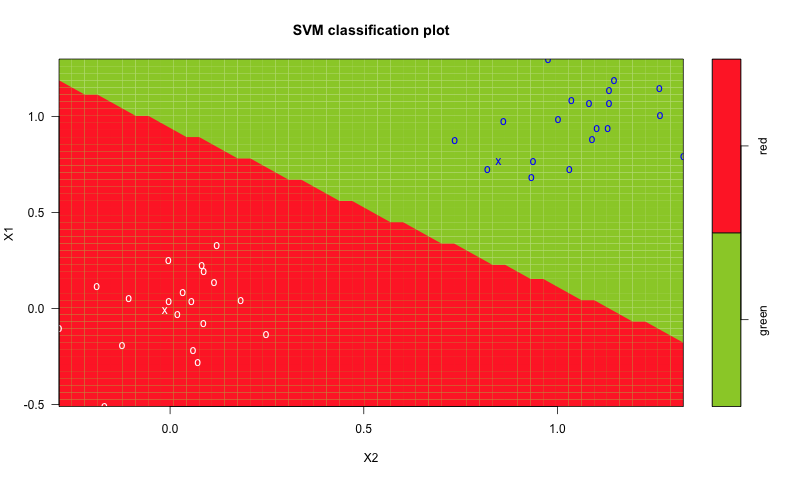
\includegraphics[width = 0.9\linewidth]{data/data1_test_set.png}
            \caption{Разбиение пространства для тестирующей выборки}
        \end{figure}

        Для были найдены ошибки классификации и количество опорных векторов (таблица 1).

        \begin{table}[H]
            \centering
            \begin{tabular}{|c|c|c|}
              \hline
              \textbf{Выборка}  & Тренирующая & Тестирующая \\
              \hline
              \textbf{Ошибка классификации} & 0.0 & 0.0\\
              \hline
              \textbf{Количество опорных векторов} & 2 & 2\\
              \hline
            \end{tabular}
            \caption{Сравнение результатов с исходными данными (<<Крестики-нолики>>)}
        \end{table}

    \section{Набор данных <<svmdata2>>}
        В качестве классификатора выбран метод опорных векторов типа <<C-classification>> с линейным ядром. Для того, чтобы добиться нулевой ошибки на обучающей выборке параметру C было присвоено значение 183. Однако, в таком случае присутствует ошибка 0.06 на тестовой выборке. Разбиение пространства для этого случая изображено ниже (рис. 3-4).

        Для того, чтобы добиться нулевой ошибки на тестирующей выборке параметру C было присвоено значение 1. Однако, в таком случае присутствует ошибка 0.02 на тренировочной выборке. Разбиение пространства для этого случая изображено ниже (рис. 5-6).

        Вообще говоря, я бы склонился к использованию параметра C = 1, так как в данном случае допустить всего одну ошибку в тренировочной выборке не так страшно, как допустить 3 ошибки в тестирующей выборке.

        \begin{figure}[H]
            \centering
            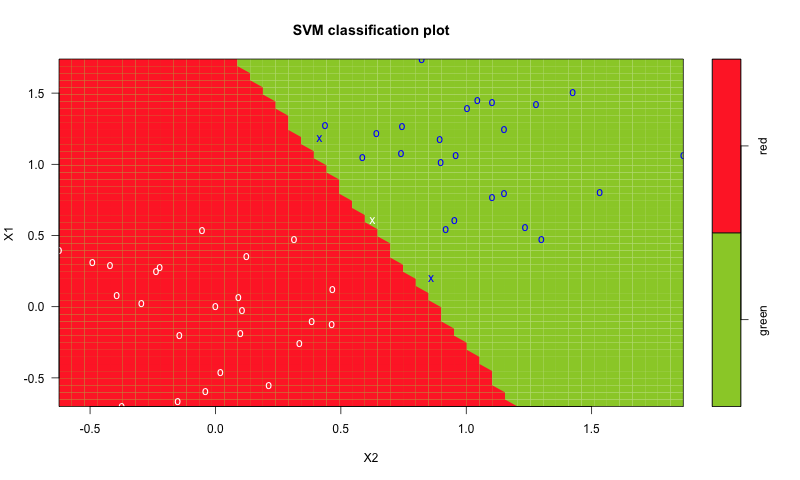
\includegraphics[width = 0.9\linewidth]{data/data2_train_set_183.png}
            \caption{Разбиение пространства для обучающей выборки с параметром C = 183}
        \end{figure}
        \begin{figure}[H]
            \centering
            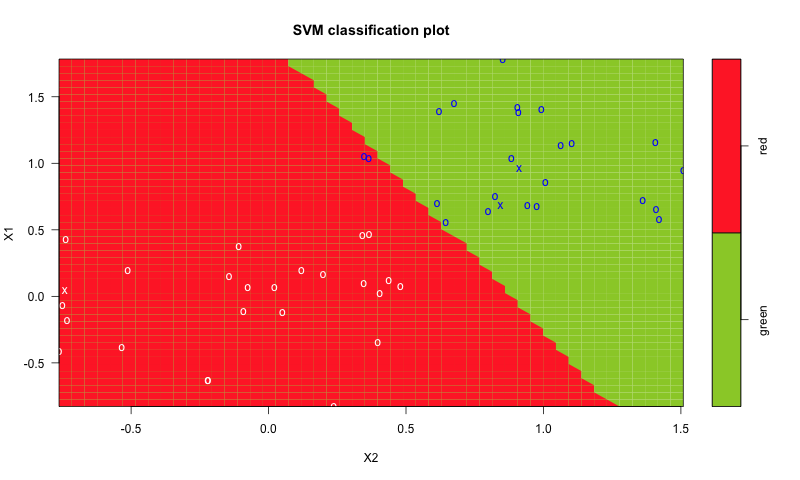
\includegraphics[width = 0.9\linewidth]{data/data2_test_set_183.png}
            \caption{Разбиение пространства для тестирующей выборки с параметром C = 183}
        \end{figure}
        \begin{figure}[H]
            \centering
            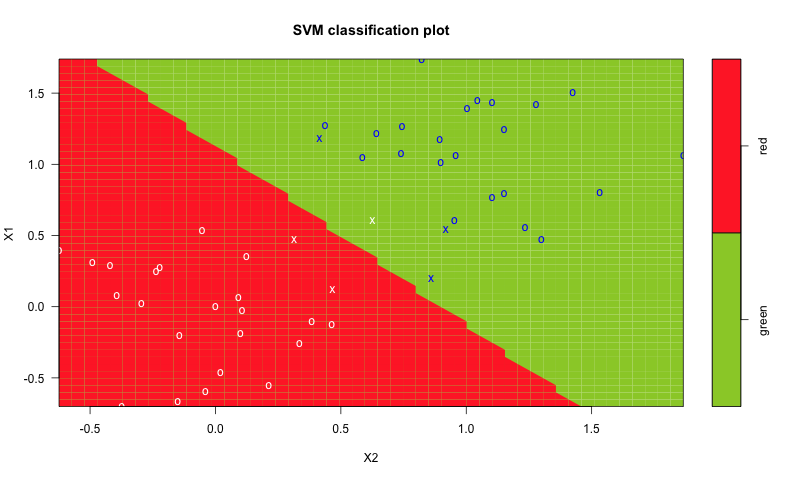
\includegraphics[width = 0.9\linewidth]{data/data2_train_set_1.png}
            \caption{Разбиение пространства для обучающей выборки с параметром C = 1}
        \end{figure}
        \begin{figure}[H]
            \centering
            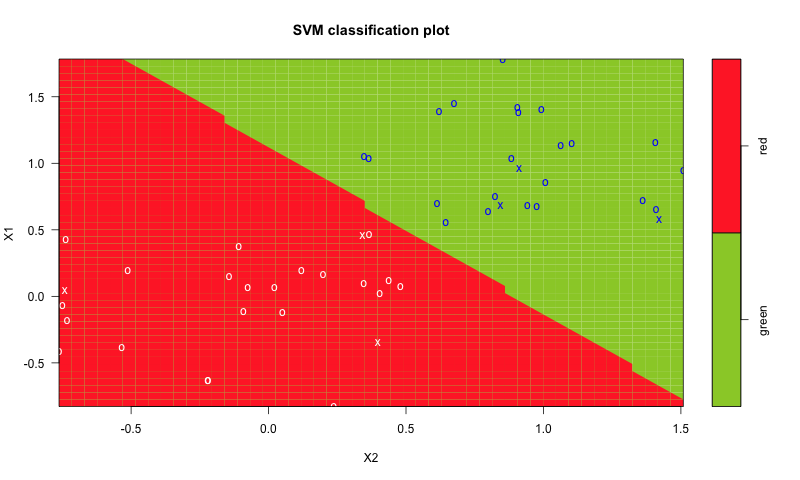
\includegraphics[width = 0.9\linewidth]{data/data2_test_set_1.png}
            \caption{Разбиение пространства для тестирующей выборки с параметром C = 1}
        \end{figure}

    \section{Набор данных <<svmdata3>>}
        На данной выборке было проведен анализ влияния параметра degree на точность предсказаний в случае полиномиального ядра (рис. 7).

        \vspace{-0.5cm}
        \begin{figure}[H]
            \centering
            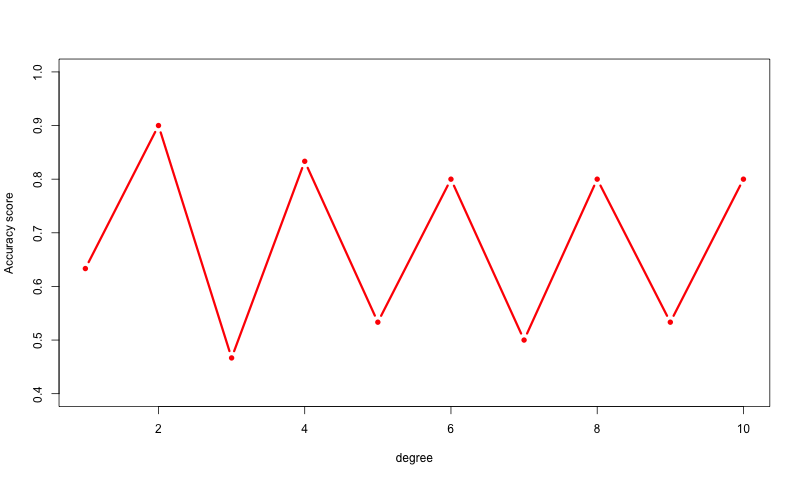
\includegraphics[width = 0.9\linewidth]{data/data3_poly_degree.png}
            \caption{Зависимость точности от параметра degree}
        \end{figure}

        Было проведено сравнение функций ядра <<polynomial>>, <<radial>> и <<sigmoid>> по количеству ошибок на тестовой выборке (таблица 2). Для типа ядра <<polynomial>> было использовано значение degree = 2 в качестве оптимального.

        \begin{table}[H]
            \centering
            \begin{tabular}{|c|c|}
                \hline
                \textbf{Ядро}  & \textbf{Точность} \\
                \hline
                <<polynomial>> & 0.9 \\
                \hline
                <<radial>> & 0.93 \\
                \hline
                <<sigmoid>> & 0.6 \\
                \hline
            \end{tabular}
            \caption{Зависимость точности от типа ядра}
        \end{table}

        Для каждого обучения были построены графики разбиения пространства для тестирующей выборки (рис. 8 - 10).

        \begin{figure}[H]
            \centering
            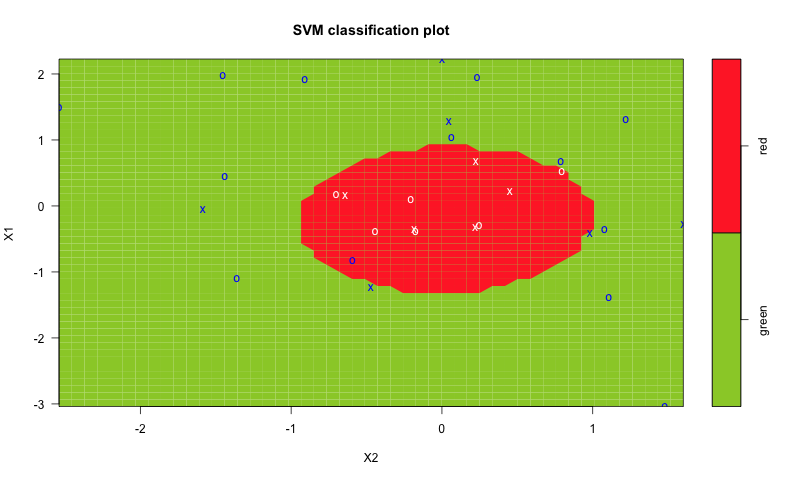
\includegraphics[width = 0.9\linewidth]{data/data3_poly.png}
            \caption{Разбиение пространства для тестирующей выборки с ядром <<polynomial>>}
        \end{figure}

        \begin{figure}[H]
            \centering
            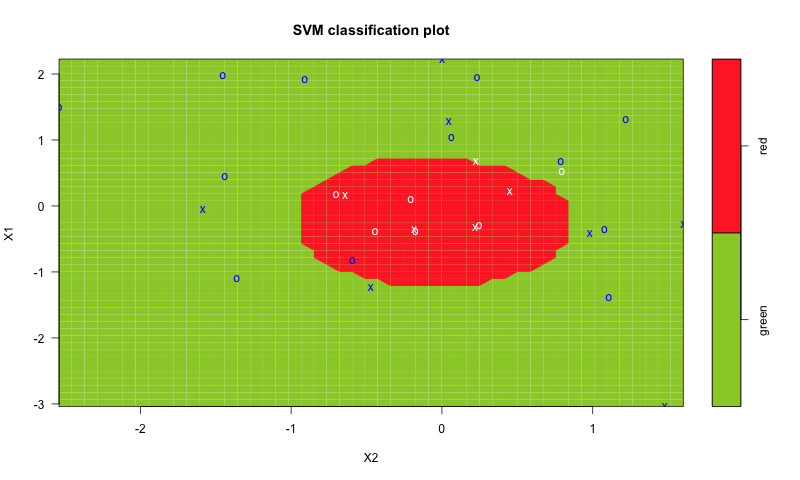
\includegraphics[width = 0.9\linewidth]{data/data3_radial.png}
            \caption{Разбиение пространства для тестирующей выборки с ядром <<radial>>}
        \end{figure}

        \begin{figure}[H]
            \centering
            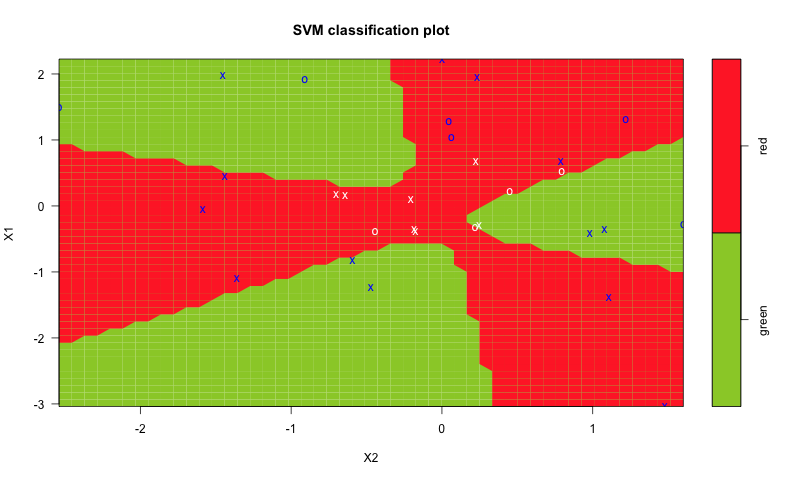
\includegraphics[width = 0.9\linewidth]{data/data3_sigmoid.png}
            \caption{Разбиение пространства для тестирующей выборки с ядром <<sigmoid>>}
        \end{figure}

    \section{Набор данных <<svmdata4>>}
        На основе метода опорных векторов построено три классификатора, которые отличаются типом ядра: <<polynomial>>, <<radial>> и <<sigmoid>>. Для тестирующей выборки была собрана информация о точности классификации для всех трех типов ядер (таблица 3 и рис. 11). Из представленных данных можно сделать вывод, что применение ядра <<radial>> наиболее уместно.

        \begin{table}[H]
            \centering
            \begin{tabular}{|c|c|}
                \hline
                \textbf{Ядро}  & \textbf{Точность} \\
                \hline
                <<polynomial>> & 0.87 \\
                \hline
                <<radial>> & 0.89 \\
                \hline
                <<sigmoid>> & 0.8 \\
                \hline
            \end{tabular}
            \caption{Зависимость точности от типа ядра}
        \end{table}

        \begin{figure}[H]
            \centering
            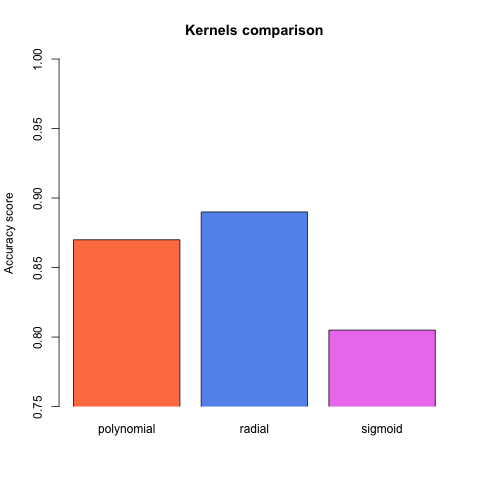
\includegraphics[width = 0.8\linewidth]{data/data4_compare_hist.png}
            \caption{Зависимость точности от типа ядра}
        \end{figure}

    \section{Набор данных <<svmdata5>>}
        На основе метода опорных векторов построено три классификатора, которые отличаются типом ядра: <<polynomial>>, <<radial>> и <<sigmoid>>. Для тестирующей выборки была собрана информация о точности классификации для всех трех типов ядер (таблица 4 и рис. 12). Из представленных данных можно сделать вывод, что применение ядра <<radial>> наиболее уместно.

        \begin{table}[H]
            \centering
            \begin{tabular}{|c|c|}
                \hline
                \textbf{Ядро}  & \textbf{Точность} \\
                \hline
                <<polynomial>> & 0.43 \\
                \hline
                <<radial>> & 0.92 \\
                \hline
                <<sigmoid>> & 0.47 \\
                \hline
            \end{tabular}
            \caption{Зависимость точности от типа ядра}
        \end{table}

        \begin{figure}[H]
            \centering
            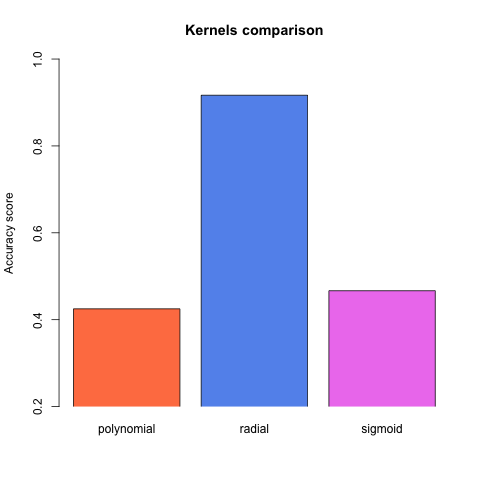
\includegraphics[width = 0.7\linewidth]{data/data5_compare_hist.png}
            \caption{Зависимость точности от типа ядра}
        \end{figure}

        Также проведено исследование влияния параметра gamma на результат обучения (рис. 13). Для дальнейшего анализа используется тип ядра  <<polynomial>>.

        \begin{figure}[H]
            \centering
            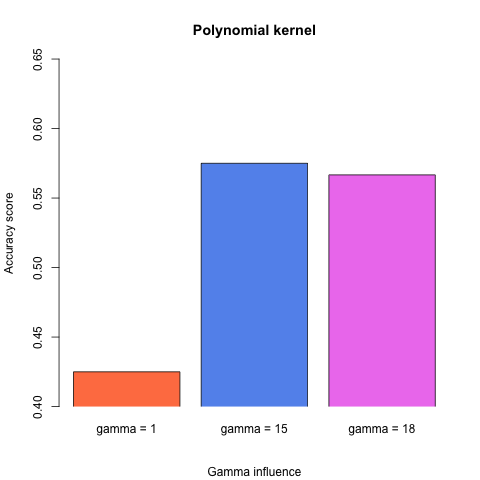
\includegraphics[width = 0.65\linewidth]{data/data5_gamma_hist.png}
            \caption{Зависимость точности от параметра gamma}
        \end{figure}
        Построены графики визуализации разбиения пространства признаков при переобучении, связанном с изменением параметра gamma (рис. 14 - 16).
        \vspace{-0.4cm}
        \begin{figure}[H]
            \centering
            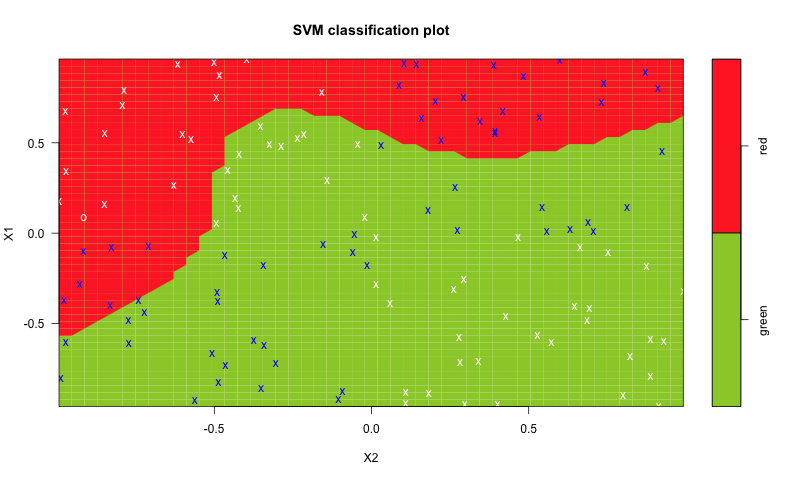
\includegraphics[width = 0.9\linewidth]{data/data5_poly_1.png}
            \caption{Разбиение пространства при gamma = 1}
        \end{figure}

        \begin{figure}[H]
            \centering
            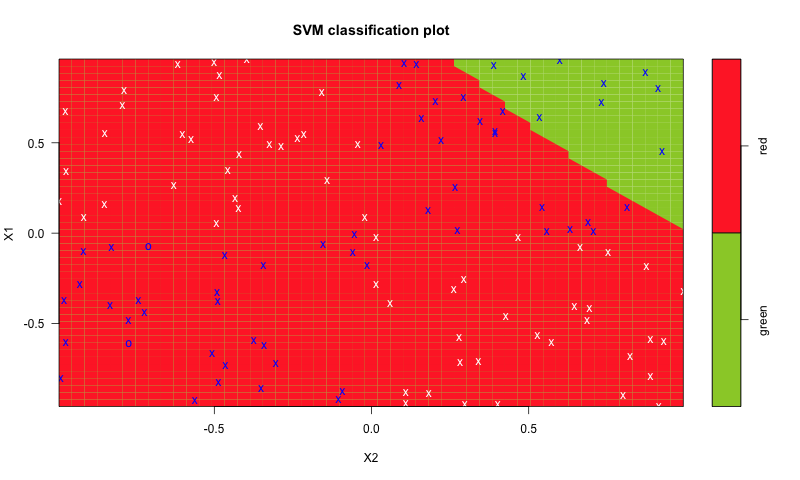
\includegraphics[width = 0.9\linewidth]{data/data5_poly_15.png}
            \caption{Разбиение пространства при gamma = 15}
        \end{figure}

        \begin{figure}[H]
            \centering
            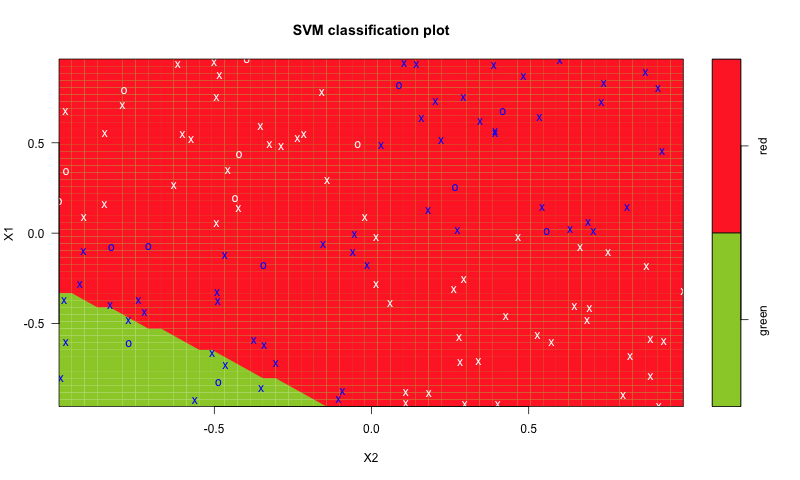
\includegraphics[width = 0.9\linewidth]{data/data5_poly_18.png}
            \caption{Разбиение пространства при gamma = 18}
        \end{figure}

    \section{Набор данных <<svmdata6>>}
        На основе метода опорных векторов типа <<eps-regression>> был построен классификатор. Построен график на котором изображена исходная выборака, опорные векторы, восстановленная зависимость и ее $\epsilon$-окрестность (рис. 17).

        \begin{figure}[H]
            \centering
            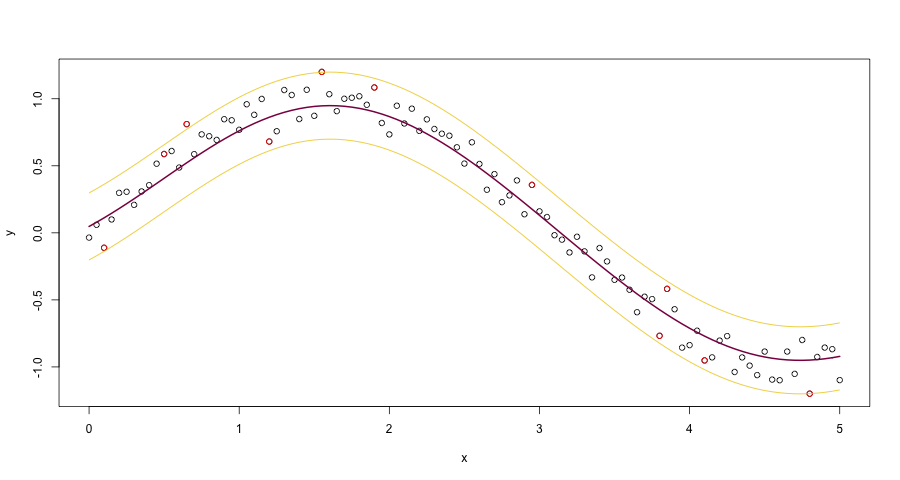
\includegraphics[width = 0.9\linewidth]{data/data6_eps.png}
            \caption{Полученные данные для набора <<svmdata6>>}
        \end{figure}

\end{document}
